%!TEX root = ../template.tex
%%%%%%%%%%%%%%%%%%%%%%%%%%%%%%%%%%%%%%%%%%%%%%%%%%%%%%%%%%%%%%%%%%%%
%% chapter4.tex
%% NOVA thesis document file
%%
%% Chapter with lots of dummy text
%%%%%%%%%%%%%%%%%%%%%%%%%%%%%%%%%%%%%%%%%%%%%%%%%%%%%%%%%%%%%%%%%%%%

\typeout{NT FILE chapter4.tex}%

\chapter{Tool Design for Blade Clearance Control}
\label{cha:toolclear}


Following the conclusions drawn in Section~\ref{cha:contacto} regarding the actual contact points between blade platforms, this chapter focuses on applying reverse engineering to determine the chord length of the blade platforms and . The approach involves analyzing the contact zones identified previously and determine the correct platform chord dimensions. Furthermore, the diameters of the spool will be determined by opening a case with the manufacturer to request these specific dimensions, ensuring accuracy in the assembly process.

With this information, the chapter proceeds to the design of a tool for blade clearance control, capable of assessing the contact clearance between the blades during assembly. The tool will be designed based on nominal tolerances, estimated blade configurations, and the dimensional analysis of the spool diameter, ensuring precise control over the final assembly clearance.


\section{Statistical Analysis for Tolerance Estimation}

The first step in this process is determining how many blades need to be measured in order to obtain a credible and accurate chord dimension. 
To assess this, a statistical methodology was applied. Since no manufacturing tolerances were provided, these were estimated based on direct measurements performed with a caliper. 
The approach is grounded in standard principles of statistical quality control and process capability analysis, as detailed in Requeijo and Pereira's work on process planning and statistical control.

\subsection{Sampling Strategy}

Building upon the methodology, the next step is to determine the number of blades to be measured from each stage to ensure reliable results. 
A pilot sample was used to estimate the required number of measurements for process characterization.
Six used blades were measured per stage using a digital caliper. The results for stages 6 to 10 are presented in Table~\ref{tab:pilot_measurements}.
As shown in Figure~\ref{fig:corda}, the dimension "x" represents the chord length being measured on the blade platform.

\begin{figure}[H]
    \centering
    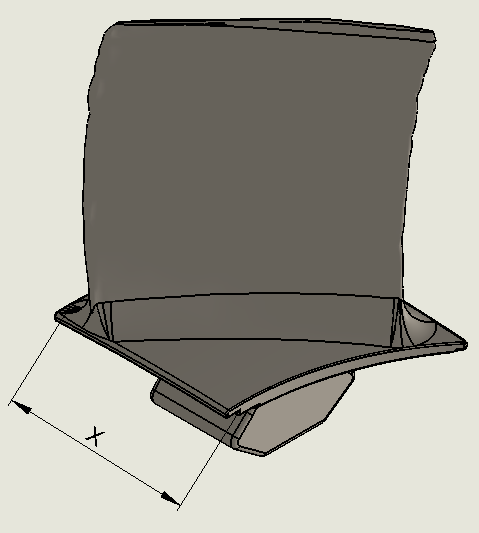
\includegraphics[width=0.4\textwidth]{corda}
    \caption{Platform blade with the chord dimension being measured, indicated as "x".}
    \label{fig:corda}
\end{figure}

\begin{table}[H]
    \centering
    \caption{Pilot measurements of platform chord lengths (mm) for stages 6 to 10.}
    \label{tab:pilot_measurements}
    \begin{tabular}{ccccc}
        \hline
        \textbf{Stg 6} & \textbf{Stg 7} & \textbf{Stg 8} & \textbf{Stg 9} & \textbf{Stg 10} \\
        \hline
        18.71 & 20.37 & 18.59 & 19.48 & 18.26 \\
        18.71 & 20.36 & 18.58 & 19.49 & 18.28 \\
        18.72 & 20.37 & 18.61 & 19.46 & 18.28 \\
        18.72 & 20.36 & 18.58 & 19.47 & 18.26 \\
        18.71 & 20.36 & 18.59 & 19.48 & 18.28 \\
        18.72 & 20.37 & 18.57 & 19.48 & 18.28 \\
        \hline
    \end{tabular}
\end{table}

Using this data, the required sample size \(n\) for a given confidence level of and measurement precision was determined using the expression:

\[
n = \left( \frac{Z \cdot s}{E} \right)^2
\]

Where:
\begin{itemize}
    \item \(Z\): standard normal value for the chosen confidence level (in this case 1.96 for 95\% of confidence),
    \item \(s\): standard deviation estimated from the pilot sample,
    \item \(E\): maximum acceptable error (typically set to 0.01 mm, matching the caliper's resolution).
\end{itemize}

The values of \(s\) and the corresponding sample sizes for each stage are presented in Table~\ref{tab:sample_sizes_data} for the narrow body type blades and on Table~\ref{tab:sample_sizes_data_wide} for the wide body type blades.

\begin{table}[H]
    \centering
    \caption{Calculated sample sizes for Narrow Body blades based on standard deviation from pilot sample, confidence level, and maximum error.}
    \label{tab:sample_sizes_data}
    \begin{tabular}{cccc}
        \hline
        \textbf{s} & \textbf{Z} & \textbf{E} & \textbf{n} \\
        \hline
        0.006956076 & 1.96 & 0.005 & 7 \\
        0.006956076 & 1.96 & 0.005 & 7 \\
        0.013319872 & 1.96 & 0.005 & 27 \\
        0.013116504 & 1.96 & 0.005 & 26 \\
        0.006558252 & 1.96 & 0.005 & 7 \\
        \hline
    \end{tabular}
\end{table}

\begin{table}[H]
    \centering
    \caption{Calculated sample sizes for Wide Body blades based on standard deviation from pilot sample, confidence level, and maximum error.}
    \label{tab:sample_sizes_data_wide}
    \begin{tabular}{cccc}
        \hline
        \textbf{s} & \textbf{Z} & \textbf{E} & \textbf{n} \\
        \hline
        0.006956076 & 1.96 & 0.005 & 7 \\
        0.006956076 & 1.96 & 0.005 & 7 \\
        0,016558774 & 1.96 & 0.005 & 42 \\
        0,010625582 & 1.96 & 0.005 & 17 \\
        0,005679613 & 1.96 & 0.005 & 5 \\
        \hline
    \end{tabular}
\end{table}


Regarding the number of measurements per blade, only one measurement was taken per blade. 
This choice is justified by the high resolution of the caliper, which is calibrated, and the repeatability of the measurement procedure, with measurements consistently performed by a single operator. 
According to principles described in the literature, and particularly by Requeijo and Pereira, when the measurement system is precise and the method is consistent, a single measurement per part is acceptable in statistical process control. 
Repeated measurements are mostly recommended when evaluating the measurement system itself (e.g., during a repeatability and reproducibility study).

\subsection{Estimating Process Tolerance}

knowing the number of measurements needed per stage, the following step is measuring new \gls{HPC} blades available on \gls{TAP}'s engine shop.
For each blade group, the sample mean \(\bar{x}\) and standard deviation \(s\) were computed. Assuming normality in the data distribution, the process tolerance can estimated as:

\[
T = 6s
\]

According to literature this range is expected to encompass approximately 99.73\% of blades, reflecting a standard tolerance interval associated with normally distributed processes.

Example for wide blades from stage 7:

\begin{itemize}
    \item Measurements: \{20.62, 20.62, 20.61, 20.62, 20.62, 20.62, 20.61\} mm
    \item Mean: \(\bar{x} = 20.6171\) mm
    \item Standard deviation: \(s = 0.00488\) mm
    \item Tolerance estimate: \(T = 0.02928\) mm
\end{itemize}

Tables~\ref{tab:mean_tolerance_narrow} and~\ref{tab:mean_tolerance_wide} present all the measurement results and estimated tolerances for each stage.

\begin{table}[H]
    \centering
    \caption{Sample mean and tolerance estimates for each stage of the Narrow Body blades.}
    \label{tab:mean_tolerance_narrow}
    \begin{tabular}{cccc}
        \hline
        \textbf{Stage} & \multicolumn{3}{c|}{\textbf{Narrow Body}} \\
        \hline
        & \textbf{Mean (\( \bar{x} \))} & \textbf{Standard Deviation (\( s \))} & \textbf{Tolerance Estimate (\( T = 6s \))} \\
        \hline
        6  &  &  &  \\
        7  & 20.374 & 0.005345 & 0.032 \\
        8  & 18.591 & 0.007863  & 0.047 \\
        9  & 19.490 & 0.006939  & 0.042 \\
        10 & 18.284 & 0.005345  & 0.032 \\
        \hline
    \end{tabular}
\end{table}

\begin{table}[H]
    \centering
    \caption{Sample mean and tolerance estimates for each stage of the Wide body blades.}
    \label{tab:mean_tolerance_wide}
    \begin{tabular}{cccc}
        \hline
        \textbf{Stage} & \multicolumn{3}{c|}{\textbf{Wide Body}} \\
        \hline
        & \textbf{Mean (\( \bar{x} \))} & \textbf{Standard Deviation (\( s \))} & \textbf{Tolerance Estimate (\( T = 6s \))} \\
        \hline
        6  & 18.984 & 0.00535 & 0.032 \\
        7  & 20.617 & 0.00488 & 0.029 \\
        8  & 18.846 & 0.0059  & 0.035 \\
        9  & 19.753 & 0.00488  & 0.029 \\
        10 & 18.534 & 0.00548  & 0.033 \\
        \hline
    \end{tabular}
\end{table}

As discussed in Section~\ref{subsec:desafios}, the tolerance allowed for each blade at each stage, as shown in Table~\ref{tab:cleareance}, is always larger than the tolerance estimated in this chapter, making it a solid and admissible estimation.

\subsection{Conversion from Chord to Arc}

Before defining the dimensions of the blade clearance control tool, it is essential to convert the measured platform chord length into the corresponding arc length, as the actual contact between the blades occurs along the circumference of the engine's spool perimeter.

Assuming a circular geometry, the relation between the chord \(c\), arc length \(a\), and radius \(R\) is given by:

\[
a = R \cdot \theta = 2R \cdot \arcsin\left( \frac{c}{2R} \right)
\]

Where:
\begin{itemize}
    \item \(c\): chord length of the platform,
    \item \(R\): radius of the stage perimeter,
    \item \(a\): arc length corresponding to that chord.
\end{itemize}

In practice, for small angles and short chords the chord and arc are approximately equal. 
However, to ensure dimensional precision in the tool design, the arc length is computed using the actual measured chord and known stage radius.

\begin{table}[H]
    \centering
    \caption{Chord and Tolerance for Each Stage (Wide and Narrow)}
    \label{tab:chord_tolerance_per_stage}
    \begin{tabular}{ccccc}
        \hline
        \textbf{Stage} & \multicolumn{2}{c}{\textbf{Wide}} & \multicolumn{2}{c}{\textbf{Narrow}} \\
        \hline
         & \textbf{Arc length (mm)} & \textbf{Tolerance (mm)} & \textbf{Arc lenght (mm)} & \textbf{Tolerance (mm)} \\
        \hline
        6 & 20.383 & 0.032 & 18.992 & 0.032 \\
        7 & 20.383 & 0.032 & 20.626 & 0.029 \\
        8 & 18.598 & 0.047 & 18.853 & 0.035 \\
        9 & 19.498 & 0.042 & 19.761 & 0.029 \\
        10 & 18.291 & 0.032 & 18.541 & 0.033 \\
        \hline
    \end{tabular}
\end{table}



\subsection{Application to Calha Inspection}

As the combination of wide and narrow blades per stage is not fixed and may vary in each assembly, it is not practical to define a single reference value for total blade row length. Instead, the effective arc length of the blades arranged in the calha is compared against a statistically determined acceptance interval.

The expected total length is given by:

\[
L = n_W \cdot \bar{x}_W + n_N \cdot \bar{x}_N
\]

The combined standard deviation is:

\[
\sigma_{\text{total}} = \sqrt{n_W \cdot s_W^2 + n_N \cdot s_N^2}
\]

The total tolerance becomes:

\[
T_{\text{total}} = 6 \cdot \sigma_{\text{total}}
\]

Therefore, the measured arc length in the calha is considered acceptable if it falls within:

\[
[L - \frac{T_{\text{total}}}{2} , \; L + \frac{T_{\text{total}}}{2}]
\]

This approach accommodates dimensional dispersion and variability in blade configurations, offering a robust verification method aligned with practical quality control strategies.


\section{Verification of Contact-Based Clearance}

To confirm that the platform clearance measured during blade assembly (as shown in Figure~6.2) results from contact occurring at the extremities of the platform profiles as identified in Section~6.1.4 it is necessary to compare the expected clearance arc with the geometric configuration of the assembly.

Given:
\begin{itemize}
    \item Diameter: $D = 394.208$ mm
    \item Perimeter: $p = \pi D = \pi \times 394.208 = 1238.441$ mm
    \item Clearance: $0.508$ mm
\end{itemize}

\subsection*{Angle and Arc Estimation}

First it is critical to understand if the clearance chord corresponds to the arc length between two blades:

\[
\text{Clearence Arc} = 0.508 \text{ mm}
\]

To find the corresponding angle $\theta$ (in radians):

\[
\text{Clearence Chord} = 2R \cdot \sin\left(\frac{\theta}{2}\right)
\]


\[
0.508 = 394.208 \cdot \sin\left(\frac{\theta}{2}\right)
\]

\[
\sin\left(\frac{\theta}{2}\right) = \frac{0.508}{394.208} = 1.28866 \times 10^{-3}
\]

\[
\frac{\theta}{2} = \arcsin(1.28866 \times 10^{-3}) \Rightarrow \theta \approx 2.5773 \times 10^{-3} \text{ rad} \approx 0.147^\circ
\]

\[
\text{Arc Lenght (mm)} = R~(\text{mm}) \cdot \theta~(\text{rad})
\]

\[
\text{Clearence Arc Lenght} = \frac{394.208}{2} \cdot 2.5773 \times 10^{-3} = 0.508 \text{ mm}
\]


Therefore it is possible to assume that chord $\approx$ arc.

\subsection*{Recalculation with Manufacturing Tolerances}

Let:
\begin{itemize}
    \item $W = Wide Body Blade Arc Lenght$ mm 
    \item $N = Narrow Body Blade Arc Lenght$ mm
    \item $Lock = Lock Blade Arc Lenght$ mm
\end{itemize}

\[
p' = p - \text{Clearance Arc Length} = 1238.441 - 0.508 = 1237.933~\text{mm}
\]


According to 

\[
1237.933 = 26W + 36N + 4 \text{Lock} \Rightarrow 1237.933 = 26(N + 0.254) + 36N + 4N
\]

\[
N = 18.7465mm
\]

Chord Lenght associated to this value:

\[
18.7465 = \frac{394.208}{2} \cdot \theta \Rightarrow \theta = 0.0951 \text{ rad}
\]

\[
\text{Chord} = 394.208 \cdot \sin\left(\frac{0.0951}{2}\right) \approx 18.7394 \text{ mm}
\]


\begin{table}[H]
    \centering
    \caption{Measured chord values (in mm) for Narrow and Wide Body blades.}
    \begin{tabular}{cccc}
        \hline
        \textbf{Narrow Body Chord} & \textbf{(mm)} & \textbf{Wide Body Chord} & \textbf{(mm)} \\ \hline
        Blade 1 & 18.73 & Blade 6 & 18.99 \\
        Blade 2 & 18.65 & Blade 7 & 18.98 \\
        Blade 3 & 18.74 & Blade 8 & 18.98 \\
        Blade 4 & 18.76 & Blade 9 & 18.99 \\
        Blade 5 & 18.72 & Blade 10 & 18.99 \\ \hline
    \end{tabular}
\end{table}